%!TEX root = ../main.tex

\chapter{The project}
\label{chp:project}
\noindent
This chapter will explain the development behind the project by starting from the fundamentals.
\section{The 3D models}
\noindent
In this section will talk about how 3D models are saved and rendered on \ac{UE}
\subsection{The OBJ file format}
\noindent
For understanding how \ac{UE} will show 3D models and how they will be stored, we must talk about their characteristics.

\begin{itemize}
    \item \textbf{Vertices:} points that describe the geometry
    \item \textbf{Faces} indicated were there is a polygon by grouping 3 or more vertices 
    \item \textbf{Normal:} there is one for each vertex that is in a face, indicates the direction to which the face is exposed, and for calculating how light is reflected
    \item \textbf{UV:} vectors that helps how a texture should be applied to the model
    \item \textbf{Vertex colors:} RGB vector that indicates a color for each vertex
\end{itemize}
\noindent
As we talked about in chapter \ref{chp:Requirements}, we will use the OBJ file format for storing files.
The React Three Fiber has a native support for OBJ, and the backend server does not need to read the file but just to manage by saving, deleting and send it via \ac{HTTP}.
Unfortunately \ac{UE} does not have a OBJ file reader usable at runtime but just an importer for what it calls static meshes (3D models that don't have moving parts).
So there is the need to build a parser OBJ to \ac{UE} custom types.\\
First we need to understand how the OBJ file format is compose of, here a general example code:\ref{code:OBJExample}

\lstinputlisting[float=h, language=Octave, caption=OBJ file example, label={code:OBJExample}]{code/exampleOBJ.txt}
\noindent
The vertices, UV and normals are simply written, instead the faces have different formats, first not always they use triangles, but also quads, this depends on how the file was exported.
For ease of use the parser will support both. The numbers of the face are the indices of vertex, indices starts from 1.
Then a face can have also the UV and normals corresponding for the vertex. For our use cases UV aren't needed, but for future-proof they are still been parsed correctly.\\
Sometime is useful to divide the 3D model in multiple objects the OBJ format represent by dividing the 3D model with a "\verb|o|".
OBJ can also divide the faces in groups by dividing them with a "\verb|g|".
Here an example of how the division works: code:\ref{code:OBJgrouping}

\lstinputlisting[float=h, language=Octave, caption=OBJ grouping, label={code:OBJgrouping}]{code/exampleOBJGrups.txt}
\noindent
The software that the surgeons are using for exporting 3D models just support groups, so will implement those, and they will become useful for rendering the model in parts.

\subsection{To unreal types}
\noindent
\ac{UE} has some custom classes for manage thing like vectors, colors... this classes other to have useful methods they also interface with the blueprint system, we can for example expose variables or functions, so we can call them at blueprint level.
This is very important so that we can interconnect the \cpp components with blueprints.\\
Unreal has a component called \verb|procedural mesh|, this component has the possibility to render a 3D model given vertices and triangles, it also has more data that you can feed to the rendered mesh such us: normals, tangents, UV, vertex colors.
It can also have collisions and a material.\\
The \verb|procedural mesh| has also the possibility to load the mesh in parts, so the parser will save the different triangles in the various groups that are defined in the file.
This will be important later for loading time.\\
Vertices are directly read and saved in an array of \verb|FVector| and normals will be saved in the same way.
Vertex colors just need to be read and put in a \verb|LinearColor| array, the object itself can be initialized with the data retrieved in the file.
UV because are 2D vectors will be saved in an array of \verb|Vector2D|.
Unfortunately there is a mismatch between how \ac{UE} manage correlation between vertices and normals respect the OBJ file standard.
Unreal needs that two arrays that contains vertices and normals, so that the vertex in the array at the position \verb|i| must have its normal in the normal array at position \verb|i|. 
This is still a trivial problem, because there's just the need to load all the normals in memory and then save them again in the correct order decided by the faces.\\
UV are being manage in the same way.
Another problem is that unreal just accept triangles and not quads, and because it is a common practice to use quads when exporting 3D models the program will convert quads in triangles, this is pretty trivial, for each quad we can divide it in two triangles.\\
Unreal also works in \verb|Z|-up coordinates that means that the \verb|Z| axis points up, there is another standard called \verb|Y|-up were the \verb|Y| axis points up, unfortunately the OBJ file format does not have any ways to reference scale or if the file is saved in \verb|Z|-up or \verb|Y|-up,
so it is important to export the file in \verb|Z|-up.\\

\begin{figure}[h]
    \centering
    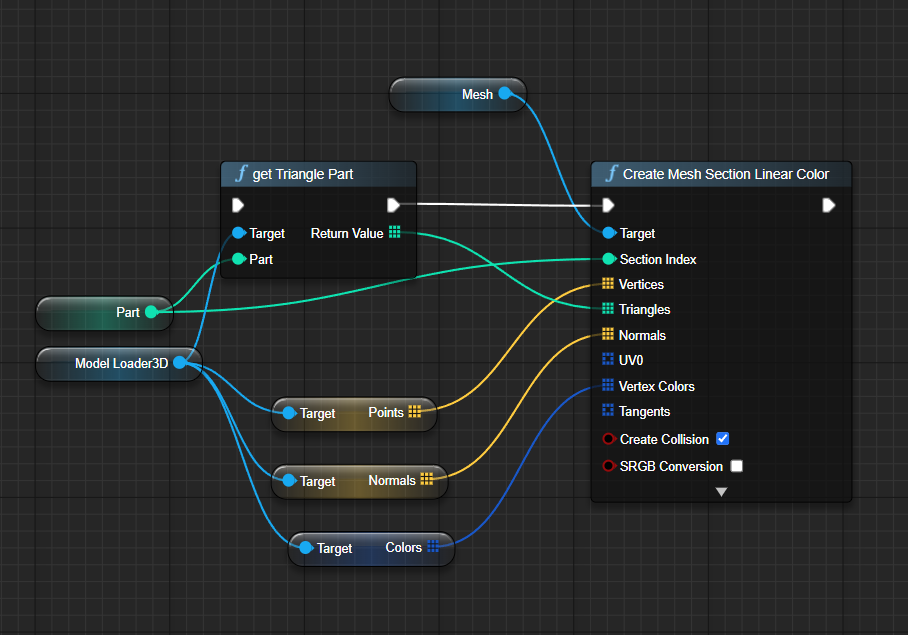
\includegraphics[width=\textwidth]{blueprints/loadingMesh.png}
    \caption{Add mesh section blueprint node}
    \label{fig:loadingMesh}
\end{figure}
\noindent
Because when loading a big procedural mesh it could create a big loss in \ac{FPS}, for reduce this problem the model will be rendered in parts, by using the different groups found on the file. After some testing I have decided to load groups every \verb|0.6ms|. 

\section{The user experience}
\noindent
Thanks to VRExpansion plugin, we can use the standard \verb|VRCharater|, this \verb*|Character| has already implemented the online synchronization, and it also has the components for the controllers and camera management.
The controllers can \verb|grip| any \verb|Actor| or \verb|Componet| that implement the interface \verb|VRGrip|, this will be used for  moving the 3D models.
Other than that the \verb|VRCharater| is an empty blank, will need to implement some functions for making fully functional.\\
Here are the main components to develop:

\begin{itemize}
    \item Input management
    \item Widget Interaction
    \item Interaction pointer
    \item Side menu
    \item Grip framework
    \item 3D model size management    
    \item Loading sphere
\end{itemize}

\subsection{Input management}
\noindent
Input in \ac{UE} is manage by two data files: \verb|Input Action |and\verb| Input Mapping Context|.
In the next two paragraphs will be addressed how the input works, and then will be used in the various components of \verb|VRCharater|.

\paragraph{Input Action}
Are files that are used to identify a certain input of the controller, each file should be named after an action more than the input used for making clear what they serve.
For example:\\
For using the \verb|A| button find in the right controller,
you need to have a file that represents the button,
the necessary settings are: Consume input which allows you to take into account that the input has been served,
and the type of value that in this case will be \verb|Digital (bool)|.

\begin{figure}[h]
    \centering
    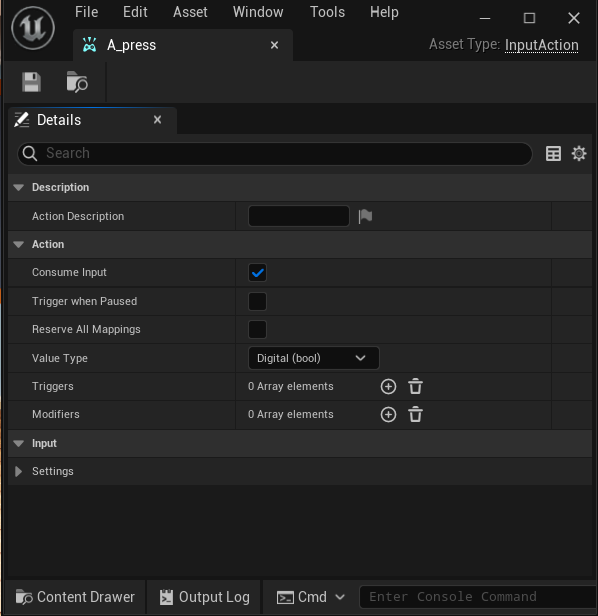
\includegraphics[width=0.7\textwidth]{blueprints/InputActionExample.png}
    \caption{Input Action example}
    \label{fig:InputAction}
\end{figure}

\paragraph{Input Mapping Context}
Each file represents all the inputs used by an actor, an actor could change its inputs, so they can be multiple files for different occasion,
Here each \verb|Input Action| will be associated with the corresponding input.
\verb|Input Mapping Context| can be used for other objects so that they can override the standard behavior of the \verb|Character|, for example by equipping a laser pointer and using the \verb|A| button for toggle it.
Each \verb|Input Mapping Context| can be bind with different controllers, this can be useful if we will be porting the app for another \ac{HMD}.
For setting the \verb|Input Mapping Context| there is a function called \verb|Add Mapping Context|.

\subsection{Widget Interaction}
\noindent 
In a normal application we are used to managing input mainly via mouse or touch screens, in \ac{VR} we can not have that, so It's important to create some kind of \ac{UI}.
One of the most used approach is showing some kind of virtual display with buttons so that the user can interact, for this will be using a blueprint called \verb|Widget| and will be explained in here ""INSERT CHAPTER"".
For letting the user see exactly were the controller is pointed, when the controller is near the \verb|Widget| a trace will be shown.
For the trace will be used a component called \verb|Spline Mesh|, as the name suggest, it uses various points and interpolate a mesh for creating a complex curve.
Still our use will be simply by just using two points. So the algorithm is simple, each tick a function called \verb|InteractionPointer| will controller for both controllers if the controller points to a \verb|Widget|, then will draw the spline.

\begin{figure}[h]
    \centering
    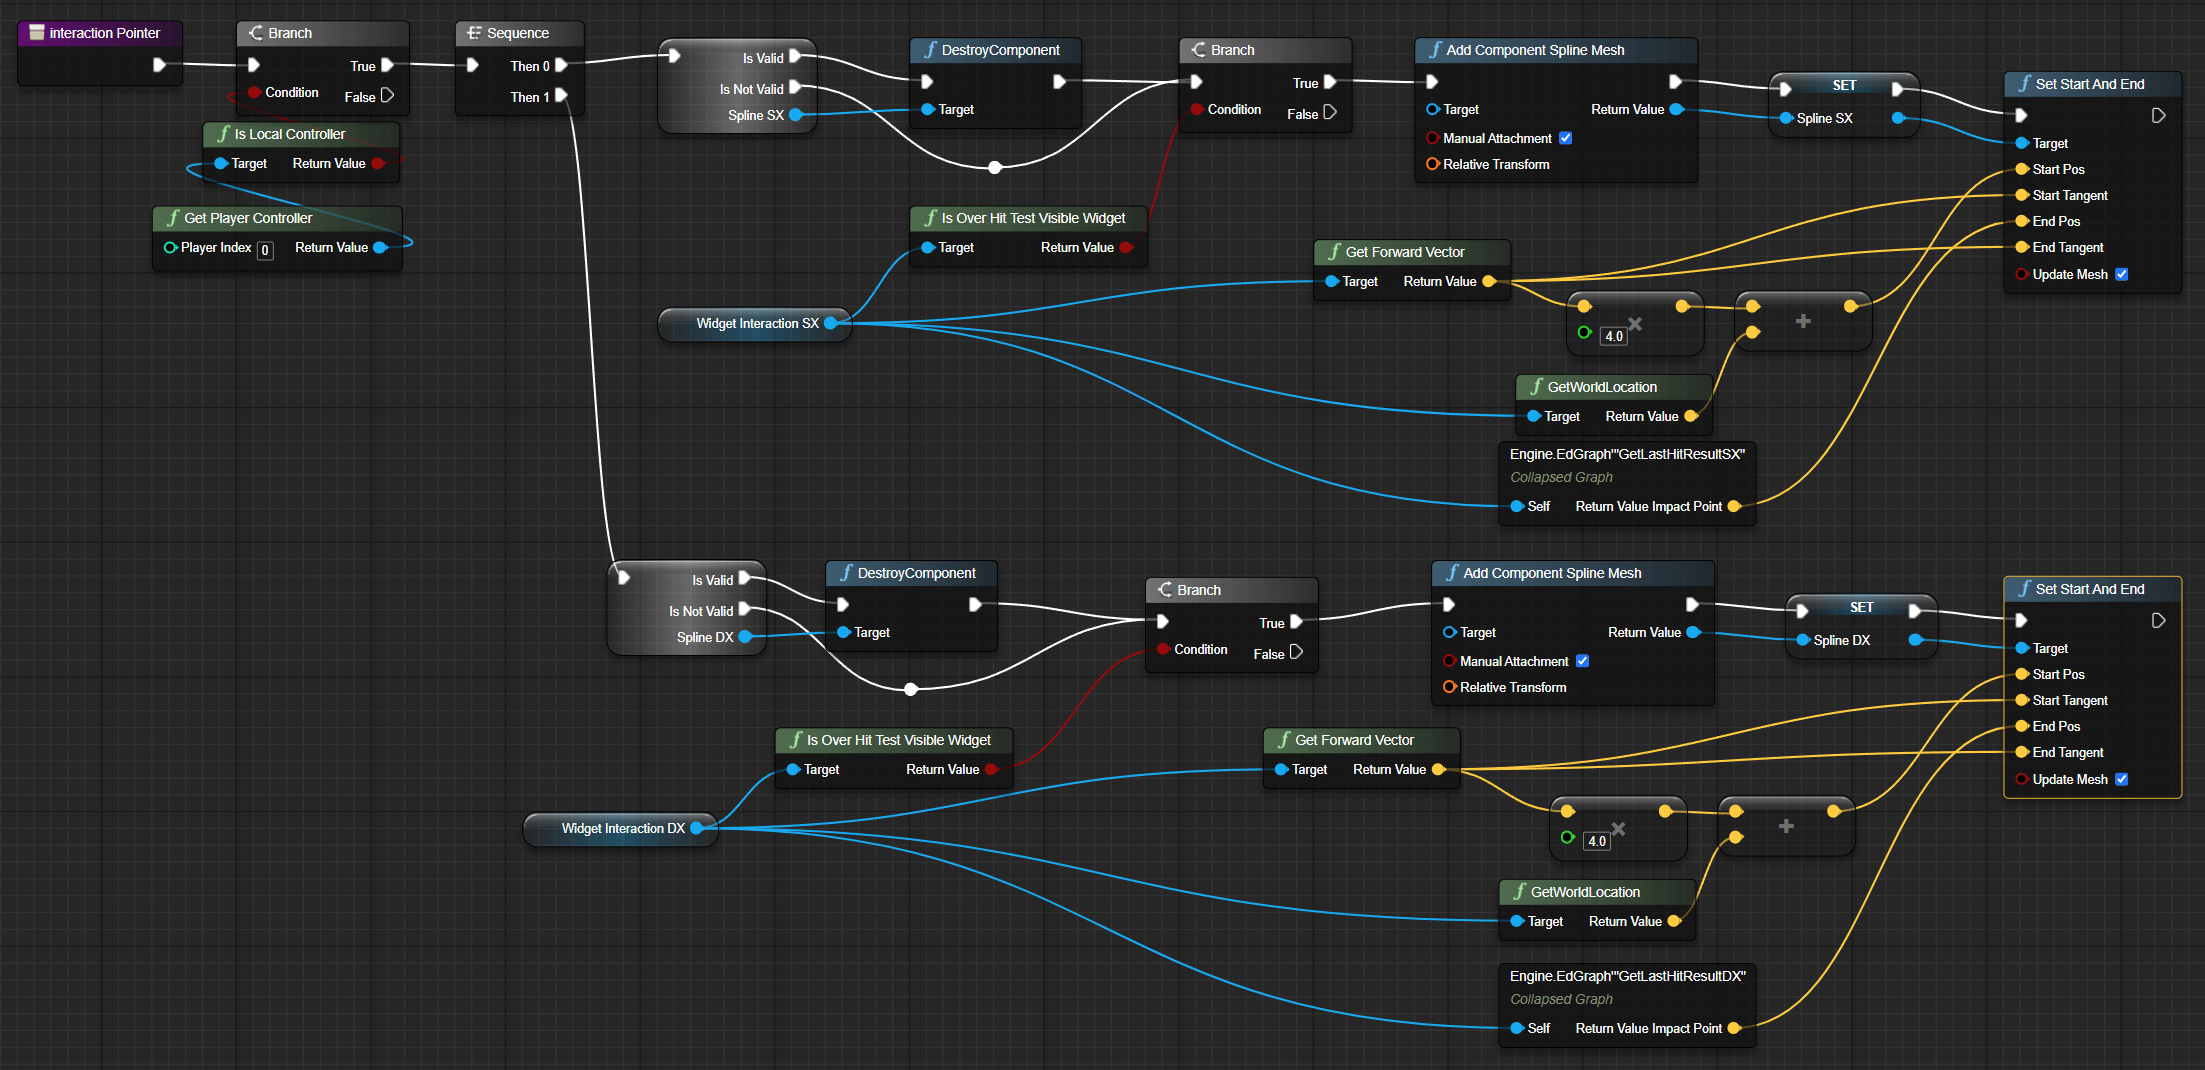
\includegraphics[width=\textwidth]{blueprints/interactionPointer.png}
    \caption{Widget Interaction code}
    \label{fig:InteractionPointer}
\end{figure}

\begin{figure}[h]
    \centering
    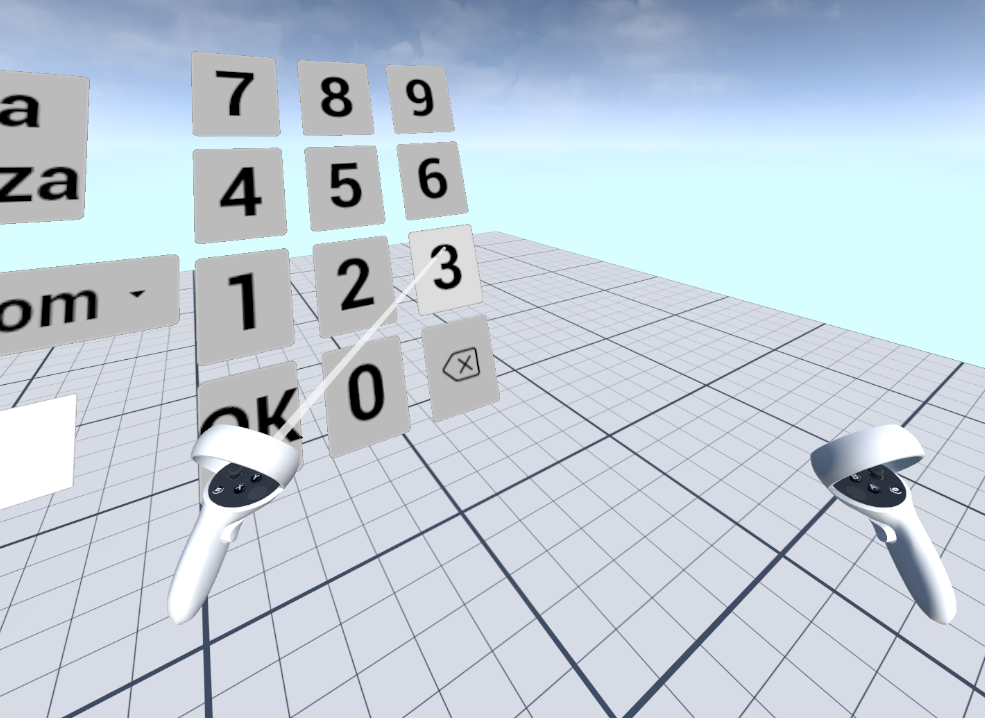
\includegraphics[width=0.8\textwidth]{vrScreenshot/splineExample.png}
    \caption{On the left a controller that create the spline pointing to the widget}
    \label{fig:splineExample}
\end{figure}